\begin{wrapfigure}{l}{0.3\linewidth}
  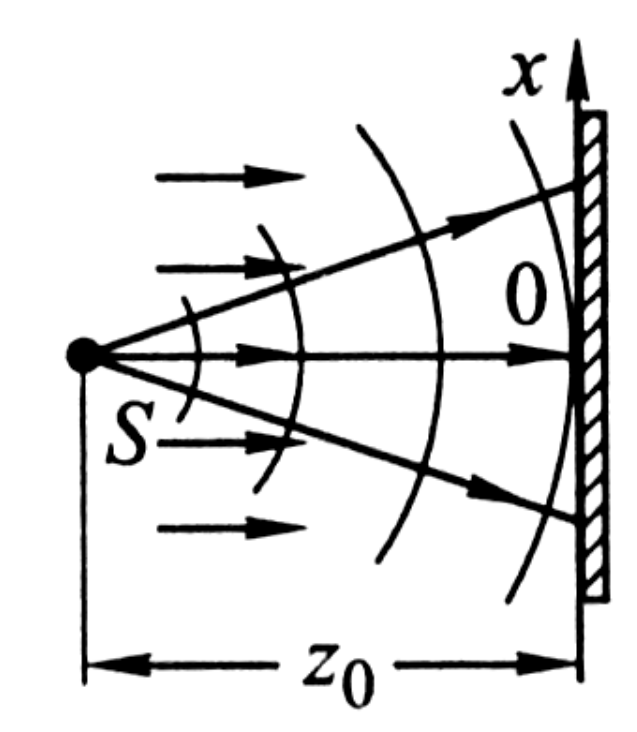
\includegraphics[width=\linewidth]{3.49.png}
  \caption{Запись голограммы точечного источника}
  \label{img::3_49}
\end{wrapfigure}

Для уяснения сути метода рассмотрим в качестве предмета точечный источник света $S$, т.~е. создадим сферическую предметную волну:

$$
f_{\Pi} = \frac{a_{\Pi}}{f} \e^{\iu kr},
$$\\
где $r = \sqrt{z_0^2 + x^2 + y^2}$ ~---~ расстояние от источника $S$ до точки $\left( x, y \right)$ фотопластинки. 

В качестве опорной волны возьмём плоскую волну, бегущую вдоль оси $z$ и падающую нормально на фотопластинку, расположенную в плоскости 
$z = 0$ (рис. \ref{img::3_49}):
$$
f_o = a \e^{\iu kz},
$$\\
т.~е. опорная волна создаёт во всех точках фотопластинки поле одинаковой амплитуды и фазы.

Принимая фазу колебаний в плоскости $z = 0$ равной нулю, запишем $f_о = a$. 
Кроме того, для упрощения формул будем далее полагать, что амплитуда сферической волны во всех точках фотопластинки равна амплитуде плоской волны, 
т.~е. $f_{\Pi} \approx a\e^{\iu kr}$. Суммарное поле в таком случае имеет вид
$$
f = a\e^{\iu kr} + \: a.
$$
\begin{wrapfigure}{r}{0.4\linewidth}
  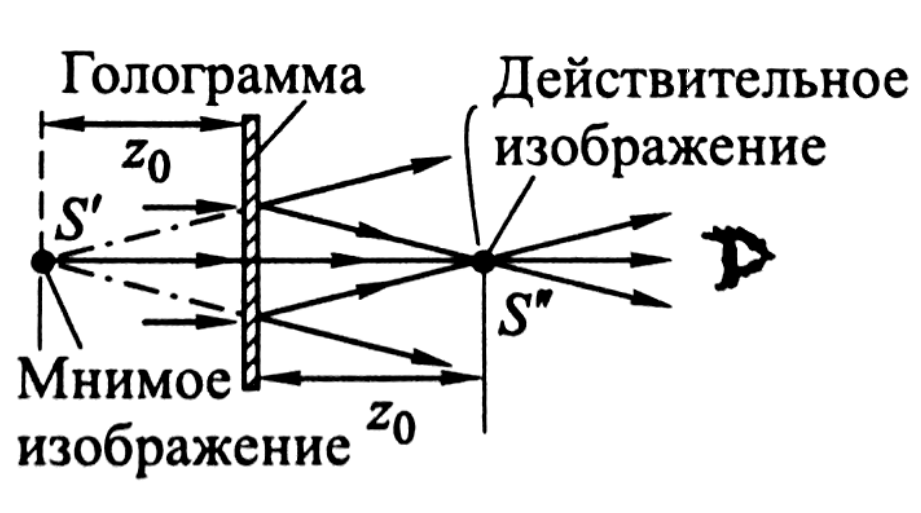
\includegraphics[width=\linewidth]{3.50.png}
  \caption{Восстановление голограммы точечного источника}
  \label{img::3_50}
\end{wrapfigure}
После необходимой фотообработки получаем голограмму с
функцией пропускания:

\begin{equation}\label{eq::3.83}
t\left(x, y\right) \sim I\left(x, y\right)  = 
\left|a +  a\e^{\iu kr}\right|^2.
\end{equation}

Мы описали первую стадию голографического процесса ~---~ процесс записи голограммы.
Теперь необходимо использовать полученную голограмму для восстановления (реконструкции) изображения.

Устанавливаем голограмму в плоскости $z = 0$ и освещаем её плоской нормально падающей волной (рис. \ref{img::3_50}). Для упрощения формул
будем считать амплитуду волны равной единице, а фазу без ограничения общности равной нулю, т.~е. комплексная амплитуда этой волны (её
называют \textbf{восстанавливающей волной}) есть $f_-(x,y) = 1$.

Тогда на выходе голограммы, в плоскости, примыкающей к ней справа, получим
\begin{equation}\label{eq::3.84}
  f_+(x,y) = f_-(x,y)t(x,y) = \left|a +  a\e^{\iu kr}\right|^2.
\end{equation}

Итак, суммарное поле за голограммой описывается действительной положительной функцией. Исследуем его более детально.

Из \eqref{eq::3.84} находим

\begin{equation}\label{eq::3.85}
  f_ +(x, y) = 2a^2 + a^2 \e^{\iu kr} + a^2 \e^{ -\iu kr} = 
  2a^2\left(1 + \cos{kr} \right)
\end{equation}

Поле в плоскости $z = 0_+$ представляется в виде суммы трёх слагаемых. Соответственно волна в области $z > 0$ есть сумма трёх волн: 
каждое слагаемое на границе $z = 0_+$ ответственно за появление \quot{своей}
волны в области $z > 0$.

Первое слагаемое $2a^2$ \quot{отвечает} за появление волны $f_1 = 2a^2\e^{\iu kz}$
~---~ плоской волны, бегущей в области $z > 0$ вдоль оси $z$. Второе слагаемое $f_2 = a^2e^{\iu kr}$ 
~---~ волновое поле со сферическим волновым фронтом:
именно такое поле создавал в каждой точке плоскости $z = 0$ точечный
источник света, который находился на расстоянии $z_0$ слева от голограммы в процессе записи. 
Ясно, что и в области $z > 0$ поле $f_2$ порождает расходящуюся сферическую волну, неотличимую от предметной волны
(сферической волны, исходящей из точки $S$ в процессе записи голограммы). 
Поэтому наблюдатель, который находится справа (в области $z > 0$) и смотрит на голограмму как в окошко, \quot{увидит в окне} на расстоянии 
$z_0$ слева от голограммы светящуюся точку $S'$, т.~е. расходящаяся сферически волна кажется наблюдателю исходящей из точки
$S'$, хотя никакой светящейся точки на стадии реконструкции изображения нет, ~---~ есть только фотопластинка-голограмма, освещаемая плоской волной. 
Это ~---~ мнимое изображение предмета.

Рассмотрим теперь последнее, третье, слагаемое в \eqref{eq::3.85}:
$f_3 = a^2\e^{-\iu kr}$. Волновой фронт в этой волне \quot{вывернут наизнанку} по отношению к волне $f_2$:
если в волне $f_2$ колебание в точке $(x,y)$ плоскости $z = 0$ отстаёт по фазе от колебаний в начале координат, то в
волне $f_3$ колебание в точке $(x,y)$ опережает по фазе колебание в начале
координат на ту же величину. Это слагаемое описывает поле, которое
создавала бы в плоскости $z = 0$ сферическая волна, сходящаяся в
точку $S''$ на расстоянии $z_0$ справа (рис. \ref{img::3_50}). 
Ясно поэтому, что граничное поле $f_3$, возникающее в процессе реконструкции, порождает сферическую волну, сходящуюся в точку $S''$. 
Это ~---~ действительное изображение предмета.
Его можно наблюдать, расположив на расстоянии $z_0$ за голограммой экран наблюдения, ~---~ мы увидим яркую точку, в которую сфокусирована волна.

Описанные закономерности сохраняются в общих чертах при голографировании произвольного предмета: в процессе реконструкции возникают три волны: волна, создающая мнимое изображение, которое
находится слева от голограммы, там же, где находился предмет при записи; волна, создающая действительное изображение, которое располагается симметрично справа от голограммы; а также волна, бегущая
вдоль оси $z$ и не несущая информации о форме волнового фронта предметной волны.
